\documentclass[tikz,border=2pt]{standalone}
\usepackage{amsmath}
\usepackage{pgfplots}
\pgfplotsset{compat=1.18}
\usetikzlibrary{arrows.meta}
\begin{document}
% Least-squares line through (0,1), (1,2), (2,2): y = 7/6 + t/2, fitted values 7/6, 5/3, 13/6,
% residuals b - A x_hat = -1/6, 1/3, -1/6 (vertical gaps), minimal sum of squares 1/6.
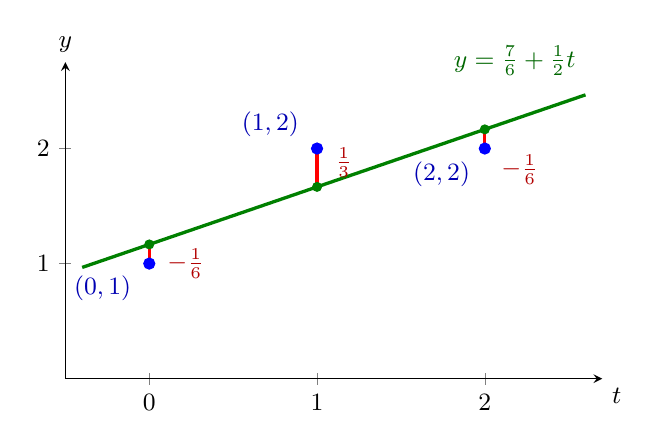
\begin{tikzpicture}[font=\small, >={Latex[length=2mm]}]
  \begin{axis}[
    axis lines=left,
    xmin=-0.5, xmax=2.7, ymin=0, ymax=2.75,
    xtick={0,1,2}, ytick={1,2},
    xlabel={$t$}, ylabel={$y$},
    xlabel style={at={(ticklabel* cs:1)}, anchor=north west},
    ylabel style={at={(ticklabel* cs:1)}, anchor=south, rotate=-90},
    clip=false,
    width=8.4cm, height=5.6cm
  ]
    \addplot[green!50!black, very thick, domain=-0.4:2.6, samples=2] {7/6+x/2};
    \node[green!40!black, anchor=south east] at (axis cs:2.6,2.55) {$y=\tfrac76+\tfrac12t$};
    % residuals
    \draw[red, very thick] (axis cs:0,1) -- (axis cs:0,7/6);
    \draw[red, very thick] (axis cs:1,2) -- (axis cs:1,5/3);
    \draw[red, very thick] (axis cs:2,2) -- (axis cs:2,13/6);
    \node[red!70!black, anchor=west] at (axis cs:0.05,1.0) {$-\tfrac16$};
    \node[red!70!black, anchor=west] at (axis cs:1.05,1.88) {$\tfrac13$};
    \node[red!70!black, anchor=north west] at (axis cs:2.04,2.03) {$-\tfrac16$};
    % fitted values and data
    \addplot[only marks, mark=*, mark size=1.6pt, green!50!black] coordinates {(0,7/6) (1,5/3) (2,13/6)};
    \addplot[only marks, mark=*, mark size=2pt, blue] coordinates {(0,1) (1,2) (2,2)};
    \node[blue!70!black, anchor=north east] at (axis cs:-0.05,0.98) {$(0,1)$};
    \node[blue!70!black, anchor=south east] at (axis cs:0.95,2.02) {$(1,2)$};
    \node[blue!70!black, anchor=north east] at (axis cs:1.97,1.97) {$(2,2)$};
  \end{axis}
\end{tikzpicture}
\end{document}
